%%%%%%%%%%%%%%%%%%%%%%%%%%%%%%%%%%%%%%%%%%%%%%%%%%%%%%%%%%%%%%%%%%%%
%% I, the copyright holder of this work, release this work into the
%% public domain. This applies worldwide. In some countries this may
%% not be legally possible; if so: I grant anyone the right to use
%% this work for any purpose, without any conditions, unless such
%% conditions are required by law.
%%%%%%%%%%%%%%%%%%%%%%%%%%%%%%%%%%%%%%%%%%%%%%%%%%%%%%%%%%%%%%%%%%%%

\documentclass[10pt]{beamer}
\usetheme[faculty=fi]{fibeamer}
\usepackage[utf8]{inputenc}
\usepackage[main=english]{babel}
\title{The wavelet scattering network for classification}
\subtitle{Introduction to wavelet scattering networks} %% title page.
\author{Hubert Leterme}
\usepackage{tikz}      % Diagrams
\usetikzlibrary{calc, shapes, backgrounds}
\usepackage{amsmath, amssymb, amsfonts, dsfont}
\usepackage{url}       % `\url`s
\usepackage{listings}  % Code listings
\usepackage[justification=centering]{caption} % Centrering captions
\frenchspacing

\newcommand{\mathN}{\mathbb{N}}
\newcommand{\mathZ}{\mathbb{Z}}
\newcommand{\mathQ}{\mathbb{Q}}
\newcommand{\mathR}{\mathbb{R}}
\newcommand{\mathC}{\mathbb{C}}

\newcommand{\MI}{{\mathcal I}}
\newcommand{\MJ}{{\mathcal J}}

\newcommand{\col}{\textcolor{yellow}}

\begin{document}

  \frame{\maketitle}

  \AtBeginSection[]{% Print an outline at the beginning of sections
    \begin{frame}<beamer>
      \frametitle{\secname}
      \tableofcontents[currentsection]
    \end{frame}}

  \begin{darkframes}
  
    \section{Introduction}
    
    \begin{frame}[label=intro]{\secname}
    \begin{itemize}
        \item One of the main tasks of image classification is to measure the level of similarity between two images.
        \item This is usually done by computing a representation for each image and then comparing the outputs, rather than directly comparing the original images.
        \item In order to build relevant classifiers, the representations must be stable under certain types of variability: translation, scaling, noise, deformations...
        \item In this presentation, we will show how to build such a representation using a wavelet scattering network, and highlight similarities with convolution neural networks.
    \end{itemize}
    \end{frame}
  
%%%%%%%%%%%%%%%%%%%%%%%%%%%%%%%%%%%%%%%%%%%%%%%%%%%%%%%%%%%%%%%%%%%%%%%%%%%%
    \section{Seeking invariant or stable representations}
    
    \subsection{Notations}
    
    \begin{frame}[label=not]{\subsecname}
    \begin{itemize}
        \item Let $\MI \subset L^2(\mathR^2)$ denote a set of input images and $\MJ \subset L^2(\mathR^2)$ a set of output image representations.
    
        For any $x \in \MI$ and $u = (u_1, u_2) \in \mathR^2$, $x(u)$ is the gray-scaled value corresponding to the position $u$.
        
        \emph{N.B.: $x$ is null outside a certain frame.}
        
        \item Let $\Phi: \MI \rightarrow \MJ$ denote a transformation which, for any $x \in \MI$, outputs a representation of $x$ denoted $\Phi x$.
        
        $\Phi x$ can have its values in $\mathR$ or in $\mathC$ (complex representations).
    \end{itemize}
    
    \end{frame}
    
    \subsection{Different types of variability}
    
    \begin{frame}[label=transl]{\subsecname}
    \framesubtitle{Global translations}
    
    \begin{columns}
    
        \column{0.6\textwidth}
        For any image $x \in \MI$ and any point $c = (c_1, c_2) \in \mathR^2$, let's denote $x_c$ the translated image with respect to $c$, i.e.:
        $$\forall u \in \mathR^2, x_c(u) = x(u-c)$$
        \col{We want: $\Phi x_c = \Phi x$.}
    
        \column{0.4\textwidth}
        
        \begin{figure}
        \centering
        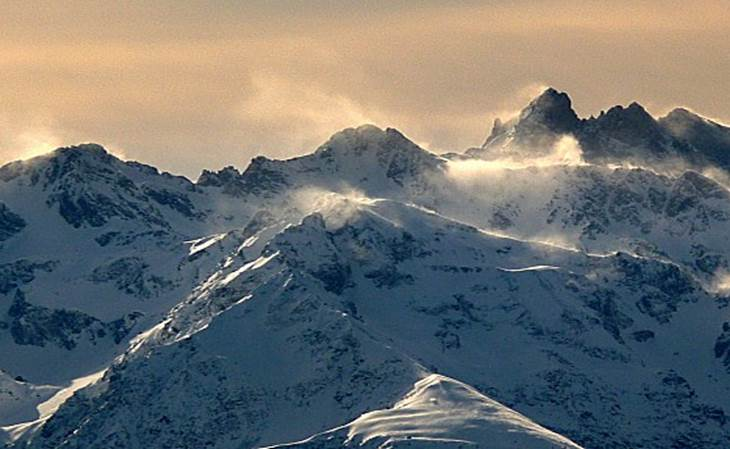
\includegraphics[height=0.3\textheight]{resources/25639-9_1.jpg}
        \vspace{0.01\textheight}
        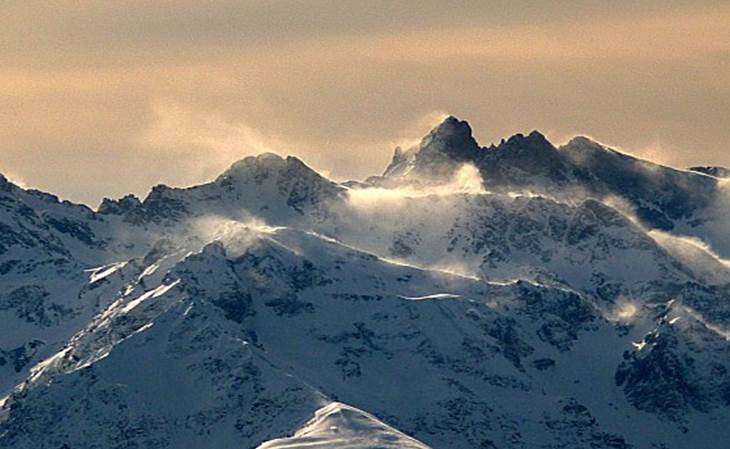
\includegraphics[height=0.3\textheight]{resources/25639-9_2.jpg}
        \end{figure}
        
    \end{columns}
    
    \end{frame}
    
    
    \begin{frame}[label=noise]{\subsecname}
    \framesubtitle{Additive noise}
    
    \begin{columns}
    
        \column{0.6\textwidth}
        For any image $x \in \MI$ and any noise $\varepsilon \in \MI$, let's denote $x'$ such that:
        $$\forall u \in \mathR^2, x'(u) = x(u) + \varepsilon(u)$$
        \col{We want $\Phi$ to be stable to additive noise:} There exists $C > 0$ such that:
        $$\forall x, x' \in \MI, \|\Phi x' - \Phi x\| \leq C \|x'-x\|$$
        (Lipschitz continuity to additive noise)
        
        \emph{N.B.: $\|.\|$ denotes the $L^2$-norm on $\MI$ and $\MJ$.} 
    
        \column{0.4\textwidth}
        
        \begin{figure}
        \centering
        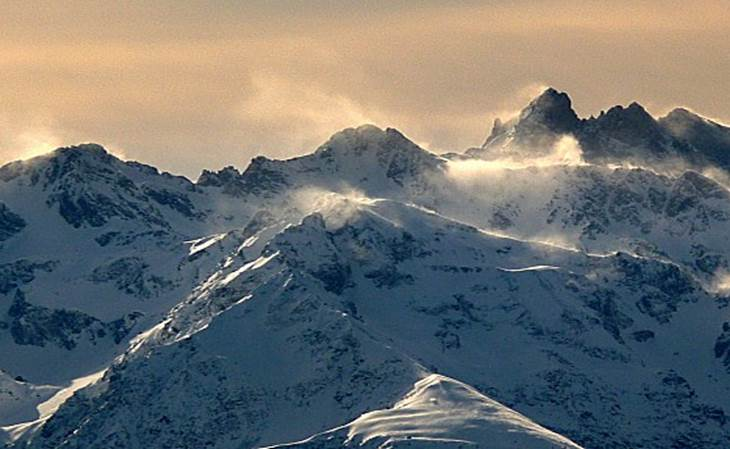
\includegraphics[height=0.3\textheight]{resources/25639-9_1.jpg}
        \vspace{0.01\textheight}
        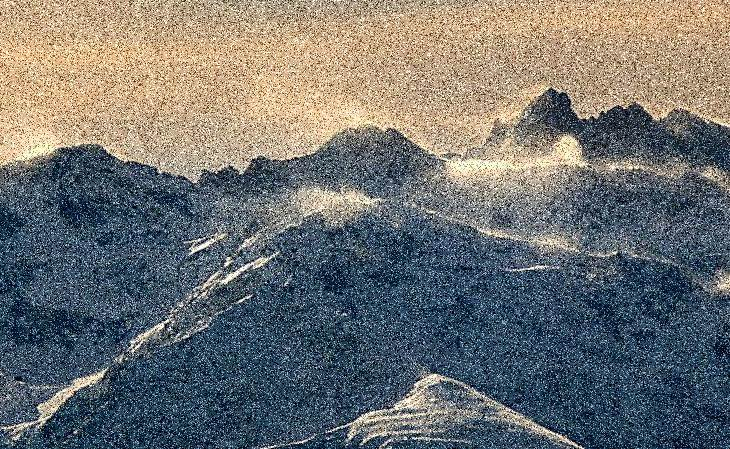
\includegraphics[height=0.3\textheight]{resources/25639-9_4.jpg}
        \end{figure}
        
    \end{columns}
    
    \end{frame}
    
    
    \begin{frame}[label=defor]{\subsecname}
    \framesubtitle{Deformations}
    \begin{columns}
        \column{0.6\textwidth}
            For any image $x \in \MI$ and any displacement field $\tau : \mathR^2 \rightarrow \mathR^2$, let's denote $x_{\tau}$ the deformed image with respect to $\tau$, i.e.:
            $$\forall u \in \mathR^2, x_{\tau}(u) = x(u-\tau(u))$$
            \col{We want $\Phi$ to be stable to deformations:} There exists $C > 0$ such that for any $x \in \MI$ and any $\tau: \mathR^2 \rightarrow \mathR^2$:
            $$\|\Phi x_{\tau} - \Phi x\| \leq C \times \|x\| \times \sup \limits_u |\nabla \tau(u)|$$
            (Lipschitz continuity to deformations)
        \column{0.4\textwidth}
            \begin{figure}
            \centering
            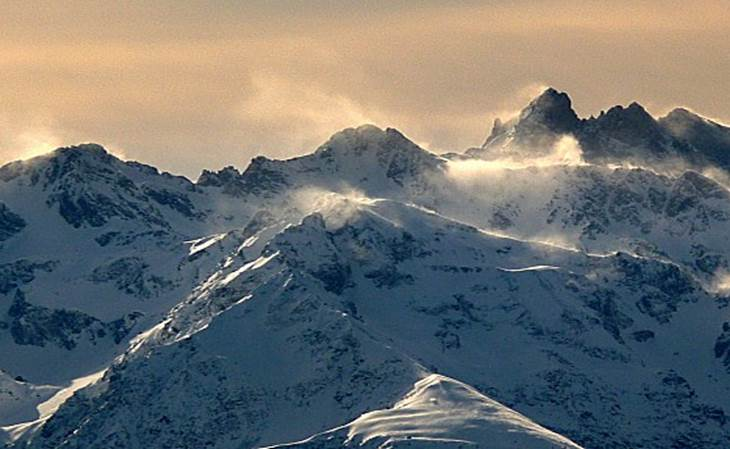
\includegraphics[height=0.3\textheight]{resources/25639-9_1.jpg}
            \vspace{0.01\textheight}
            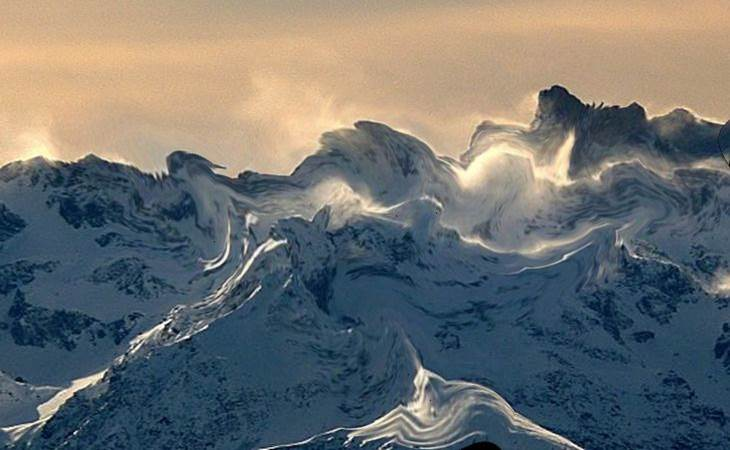
\includegraphics[height=0.3\textheight]{resources/25639-9_5.jpg}
            \end{figure}
    \end{columns}
    \end{frame}
    
    
    \begin{frame}[label=scal]{\subsecname}
    \framesubtitle{Scaling: a special kind of deformation}
    \begin{columns}
        \column{0.6\textwidth}
            For any image $x \in \MI$ and any scale factor $\alpha \in \mathR_+^*$, let's denote $x_{\alpha}$ the scaled image with respect to $\alpha$, i.e.:
            $$\forall u \in \mathR^2, x_{\alpha}(u) = x(\alpha^{-1}u)$$
        \column{0.4\textwidth}
            \begin{figure}
            \centering
            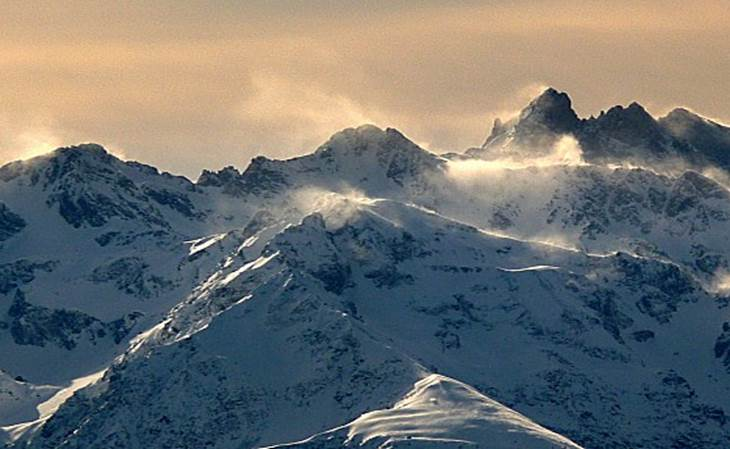
\includegraphics[height=0.3\textheight]{resources/25639-9_1.jpg}
            \vspace{0.01\textheight}
            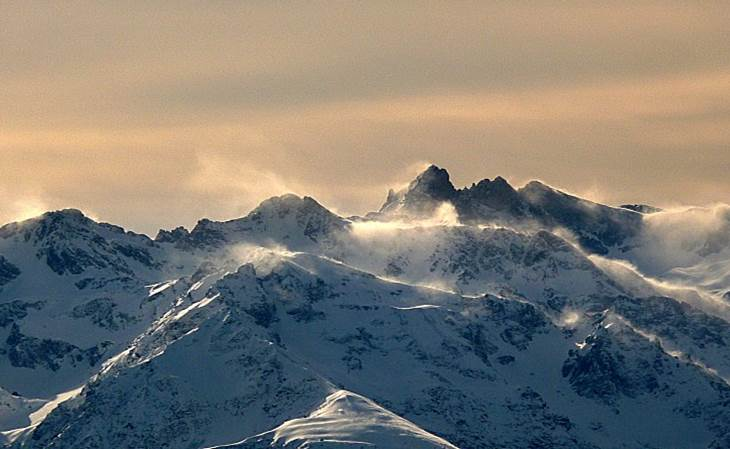
\includegraphics[height=0.3\textheight]{resources/25639-9_3.jpg}
            \end{figure}
    \end{columns}
    \end{frame}
    

    \begin{frame}[label=stable]{\subsecname}
    \framesubtitle{Why stable and not invariant representations?}
    \begin{columns}
        \column{0.5\textwidth}
            \begin{center}
            \textbf{Additive noise}
            \begin{figure}
            \centering
            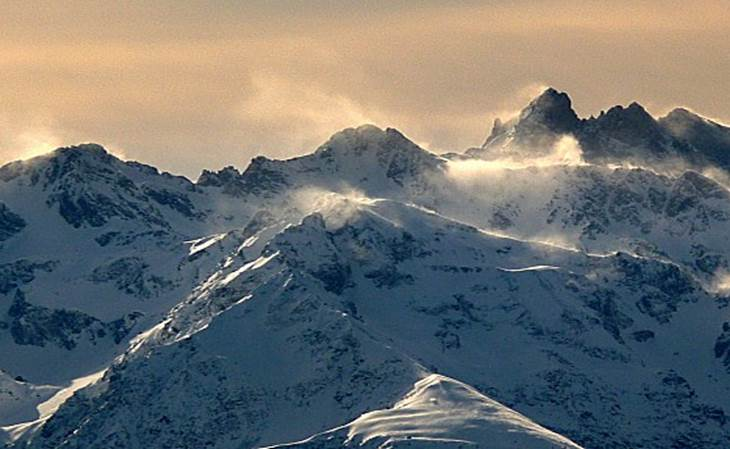
\includegraphics[height=0.25\textheight]{resources/25639-9_1.jpg}
            
            $\Downarrow$ \vspace{0.01\textheight}
            
            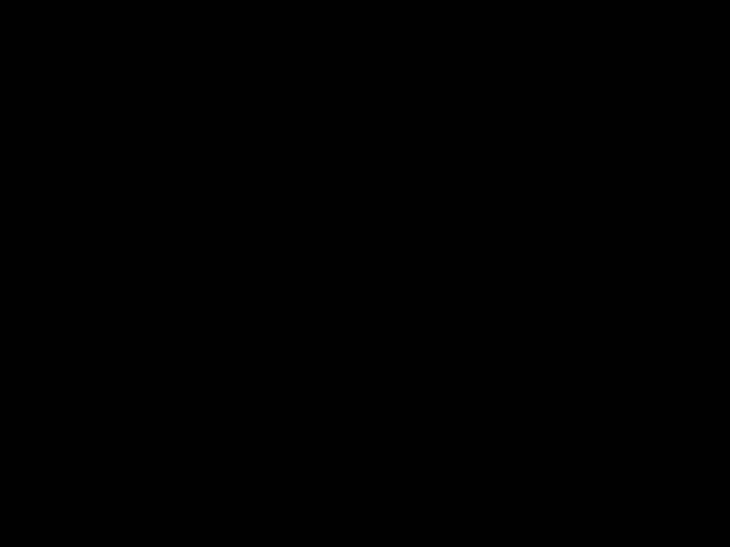
\includegraphics[height=0.25\textheight]{resources/25639-9_6.jpg}
            \end{figure}
            \end{center}
        
        \column{0.5\textwidth}
            \begin{center}
            \textbf{Deformations}
            \begin{figure}
            \centering
            
\includegraphics[height=0.25\textheight]{resources/dig1.jpg}
            
            $\Downarrow$ \vspace{0.01\textheight}
            
            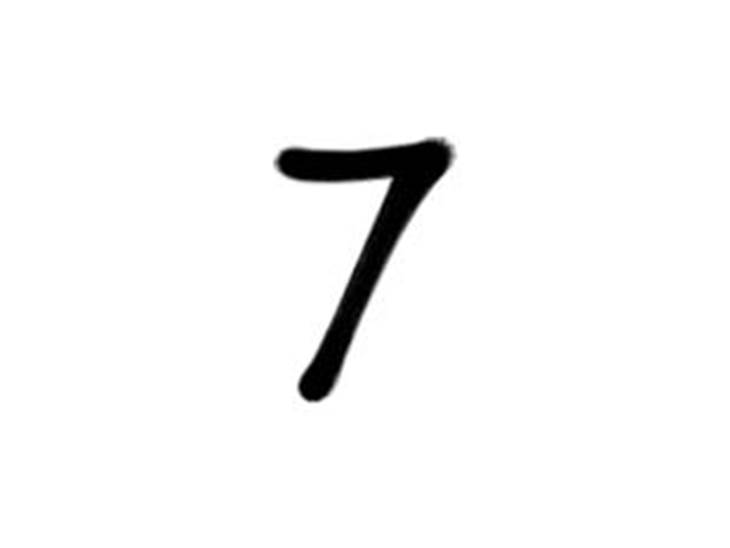
\includegraphics[height=0.25\textheight]{resources/dig7.jpg}
            \end{figure}
            \end{center}
    \end{columns}
    \end{frame}
    
    \subsection{The wavelet transform}
    
    \begin{frame}[label=repr]{\subsecname}
    \framesubtitle{Among other representations}
    \begin{small}
    \begin{center}
    \renewcommand{\arraystretch}{1.5}
    \begin{tabular}{|l|c|*{3}{c}|}
        \hline
            \multicolumn{1}{|c|}{Representation} & Formula & T & N & D \\
        \hline
            Canonical &
            $\Phi x (u) = x(u-a(x))$ &
            \checkmark & ? & X \\
            Fourier &
            $\Phi x (\omega) = \left| \iint_{\mathR^2} x(v) e^{-2i\pi \langle \omega, v \rangle}dv \right|$ &
            \checkmark & \checkmark & X \\
            Autocorrelation &
            $\Phi x (u) = \iint_{\mathR^2} x(v)x(v-u)dv$ &
            \checkmark & \checkmark & X \\
            Wavelet &
            $\Phi_\lambda x (u) = \iint_{\mathR^2} x(v) \overline{\psi_\lambda(u-v)} dv$ &
            X & \checkmark & \checkmark \\
        \hline
    \end{tabular}
    \end{center}
    \end{small}
    
    \begin{itemize}
        \item Under certain conditions, \col{the wavelet transform is stable to deformations}, unlike the others. For instance, the Fourier transform becomes unstable at high frequencies, even for small deformations.
        \item \col{Problem: the wavelet transform isn't translation-invariant}. This can be solved by introducing some non-linear transformation.
    \end{itemize}
    
    \end{frame}
    
    \begin{frame}[label=def_wavelet]{\subsecname}
    \framesubtitle{Definition}
    A function $\psi \in L^1(\mathR^2) \cap L^2(\mathR^2)$ is a \col{wavelet} ("small wave") if it satisfies the \emph{admissibility condition}:
    $$C_\psi = \iint_{\mathR^2} \frac{\left| \widehat{\psi}(\omega) \right|^2}{|\omega|} d\omega < +\infty$$
    where $\widehat{\psi}$ is the 2-dimensional Fourier transform of $\psi$.
    
    \begin{columns}
        \column{0.6\textwidth}
            \begin{itemize}
                \item Important property:
            \end{itemize}
            $$\iint_{\mathR^2} \psi(u) du = 0$$
            \begin{itemize}
                \item Example: complex Morlet wavelet:
            \end{itemize}
            $$\psi(u) = \alpha (e^{iu.\xi} - \beta) e^{-|u|^2/(2\sigma^2)}$$
        \column{0.4\textwidth}
            \begin{figure}
            \centering
            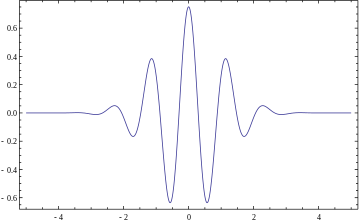
\includegraphics[width=0.8\textwidth]{resources/wavelets/360px-MorletWaveletMathematica.png}
            \caption{1D real Morlet wavelet (source: Wikipedia)}
            \end{figure}
    \end{columns}
    \end{frame}
    
    
    \begin{frame}[label=dil_rot_wavelet]{\subsecname}
    \framesubtitle{Dilated and rotated wavelets}
    From a primary wavelet $\psi$ as previously defined, we will build a \col{family of wavelets} that are \col{rotated and dilated}.
    
    Let $G$ be a group of rotations in $\mathR^2$. Then, for any $\lambda = 2^{-j} r$ such that $r \in G$ (2D-rotation matrix) and $j \in \mathZ$ ($2^{-j}$ is a dilating coefficient), we denote:
    $$\psi_\lambda(u) = 2^{-2j} \psi(2^{-j} r^{-1} u)$$
    \begin{figure}
        \centering
        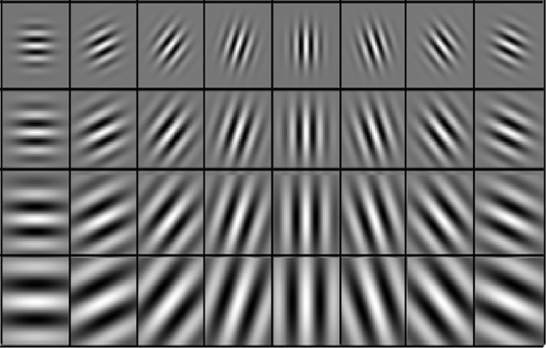
\includegraphics[width=0.5\textwidth]{resources/wavelets/Dilates_rotated_wavelets.jpg}
        \caption{Dilated and rotated wavelets (source: Naver Labs)}
    \end{figure}
    \end{frame}
    
    
    \begin{frame}[label=wavelet_trsf]{\subsecname}
    \framesubtitle{Application to image processing}
    Let $x \in \MI$. For any parameter $\lambda$ such as described before, we define the \col{wavelet transform $\Phi_\lambda x$} which is the \emph{convolution product} of $x$ and $\psi_\lambda$:
    $$\Phi_\lambda x (u) = \iint_{\mathR^2} x(v) \overline{\psi_\lambda(u-v)} dv = (x \ast \psi_\lambda)(u)$$
    \begin{itemize}
        \item One can show that this representation is \col{stable and invertible} if the wavelet filters $\widehat{\psi}(\omega)$ cover the whole frequency plane (see next slide).
        \item Since the wavelet quickly decreases to $0$, in the output representation, the value at each point is only influenced by its vicinity. For this reason, \col{the wavelet transform is not translation-invariant}.
    \end{itemize}
    \end{frame}
    
    \begin{frame}[label=fourier]{\subsecname}
    \framesubtitle{The wavelets in the Fourier domain} 
    \begin{columns}
        \column{0.4\textwidth}
            This figure displays the support of dilated (3 dilation factors) and rotated (12 rotations) wavelets in the Fourier domain.
            
            The wavelet transforms act like \col{band-pass filters.}
            
            {\emph N.B.: The smaller the support, the more dilated the wavelet ("uncertainty principle").}
        \column{0.6\textwidth}
            \begin{figure}
            \centering
            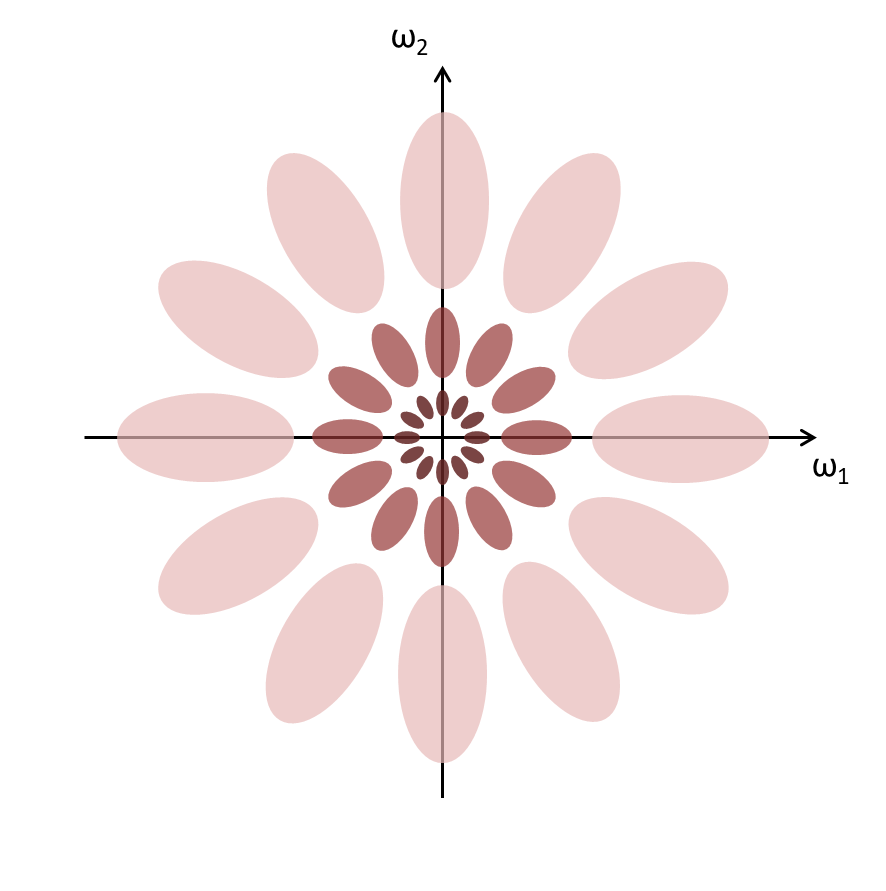
\includegraphics[width=0.9\textwidth]{resources/wavelets/Fourier_domain.png}
            \caption{Support of $\widehat{\psi}_{2^{-j}r}(\omega)$}
            \end{figure}
    \end{columns}
    \end{frame}
    
    
    \begin{frame}[label=conv_ex]{\subsecname}
    \framesubtitle{Illustration of a convolution product}
    \begin{figure}
        \centering
        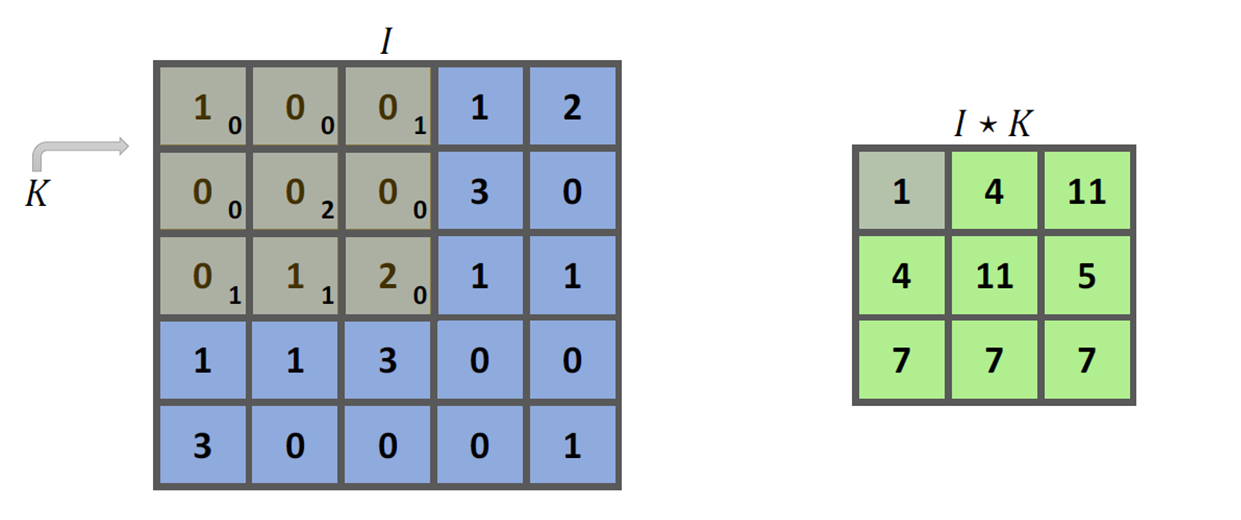
\includegraphics[width=0.40\textwidth]{resources/convolution/Conv_1.png}
        \hspace{0.01\textwidth}
        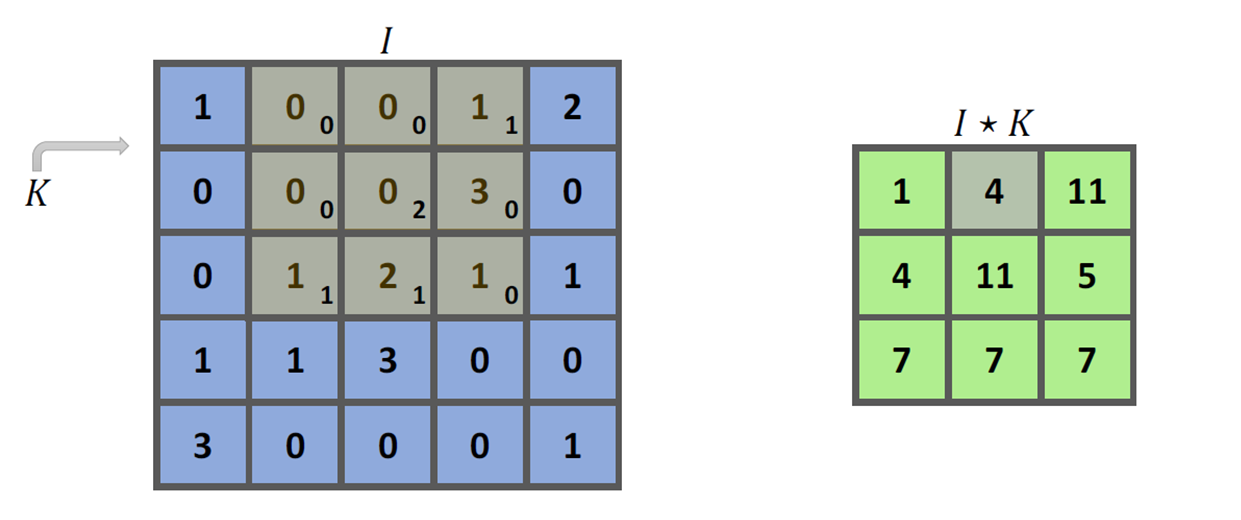
\includegraphics[width=0.40\textwidth]{resources/convolution/Conv_2.png}
        \vspace{0.015\textheight}
        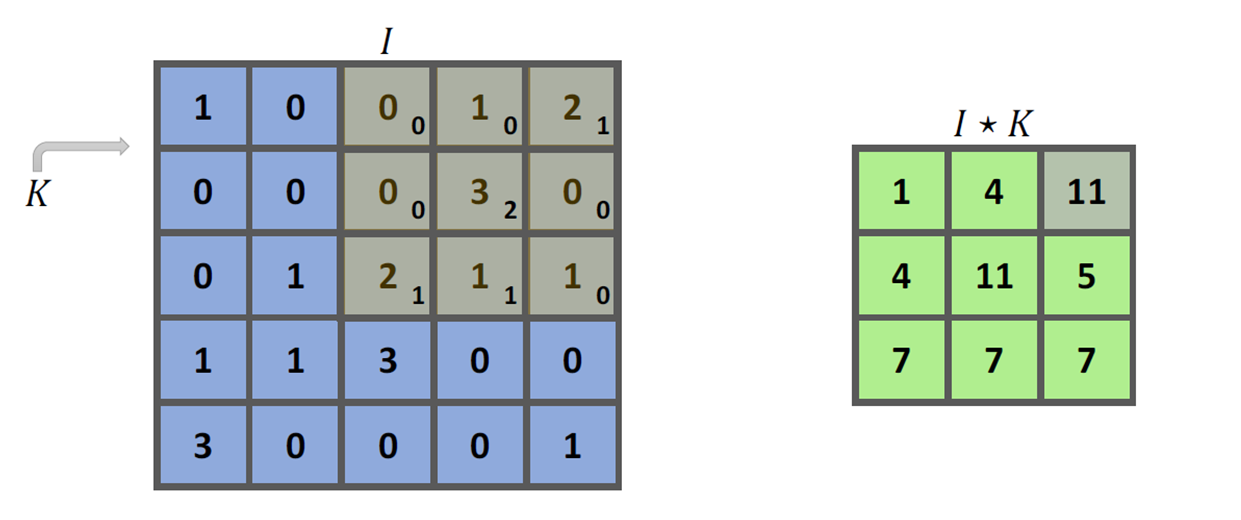
\includegraphics[width=0.40\textwidth]{resources/convolution/Conv_3.png}
        \caption{Discrete convolution product (source: Naver Labs)}
    \end{figure}
    In this example, the blue matrix $I$ can be seen as the input image and the grey matrix $K$ can be seen as the wavelet.
    \end{frame}
    
    
    \subsection{Introducing non-linearity}
    
    
    \begin{frame}[label=non-lin1]{\subsecname}
    \framesubtitle{Requirements}
    If an operator $Q$ (not necessarily linear) commutes with translations, we can prove that $\left( x \mapsto \int Qx(u) du \right)$ is translation-invariant.
    
    Since the wavelet transform commutes with translation, we could use this result to build a translation-invariant operator. Unfortunately in that case, $\int \Phi_\lambda x(u) du$ always outputs $0$, which is totally useless for classification.
    
    \vspace{6pt}
    \col{$\Rightarrow$ The idea is to seek a non-linear operator $M$ such that:}
    \begin{itemize}
        \item $M \circ \Phi_\lambda$ also commutes with translations
        \item $x \mapsto \int (M \circ \Phi_\lambda) x(u) du$ is stable to deformations and additive noise
        \item $M$ preserves the signal energy
    \end{itemize}
    \end{frame}
    
    \begin{frame}[label=non-lin2]{\subsecname}
    \framesubtitle{The $L^1$ norm}
    In order to meet these requirements, we can choose $M$ equal to the modulus operator. For any $x \in \MI$, $u \in \mathR^2$:
    $$(M \circ \Phi_\lambda) x(u) = M(x \ast \psi_\lambda)(u) = |x \ast \psi_\lambda(u)|$$
    By integrating this quantity, we get the $L^1$-norm:
    $$\|x \ast \psi_\lambda\|_1 = \int |x \ast \psi_\lambda(u)| du$$
    \col{$\Rightarrow$ The $L^1$-norm of a wavelet transform is a representation which is translation-invariant and stable to additive noise and deformations.}
    \end{frame}
    
%%%%%%%%%%%%%%%%%%%%%%%%%%%%%%%%%%%%%%%%%%%%%%%%%%%%%%%%%%%%%%%%%%%%%%%%%%%%
    \section{Toward a convolution network}
    
    \subsection{Definition}

    \begin{frame}[label=def_conv]{\subsecname}
    $\implies$ Sebastian's presentation
    \end{frame}
    
    \subsection{The wavelet scattering network}
    
    \begin{frame}{\subsecname}
    \framesubtitle{First convolution}
    In the previous section, we have implicitly built a convolutional neural network with 2 layers (providing images are discretized). Given a parameter $\lambda$, we have the following CNN:
    \end{frame}
    
    \begin{frame}{\subsecname}
    \framesubtitle{First convolution}
    \begin{figure}
        \centering
        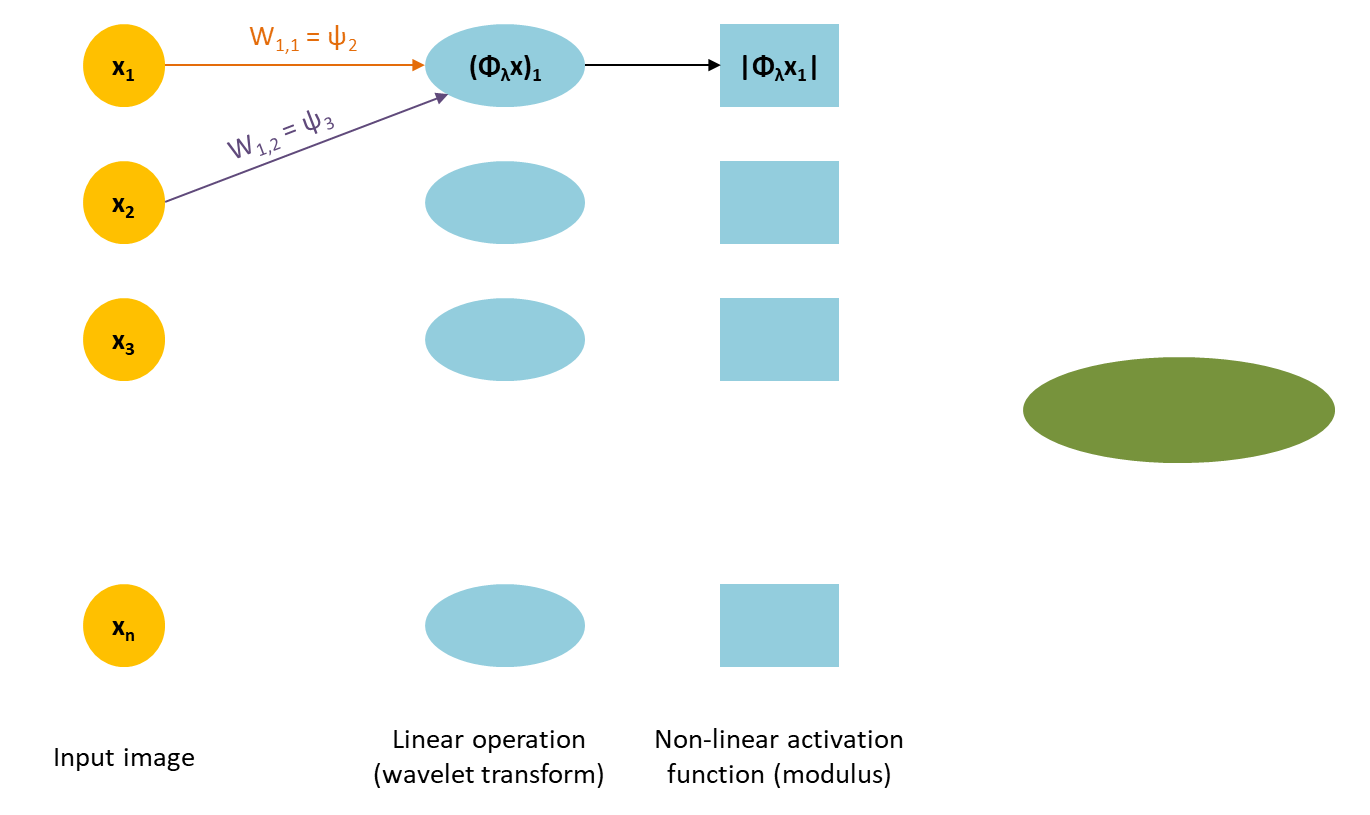
\includegraphics[width=\textwidth]{resources/convolution/CNN1.png}
    \end{figure}
    \end{frame}
    
    \begin{frame}{\subsecname}
    \framesubtitle{First convolution}
    \begin{figure}
        \centering
        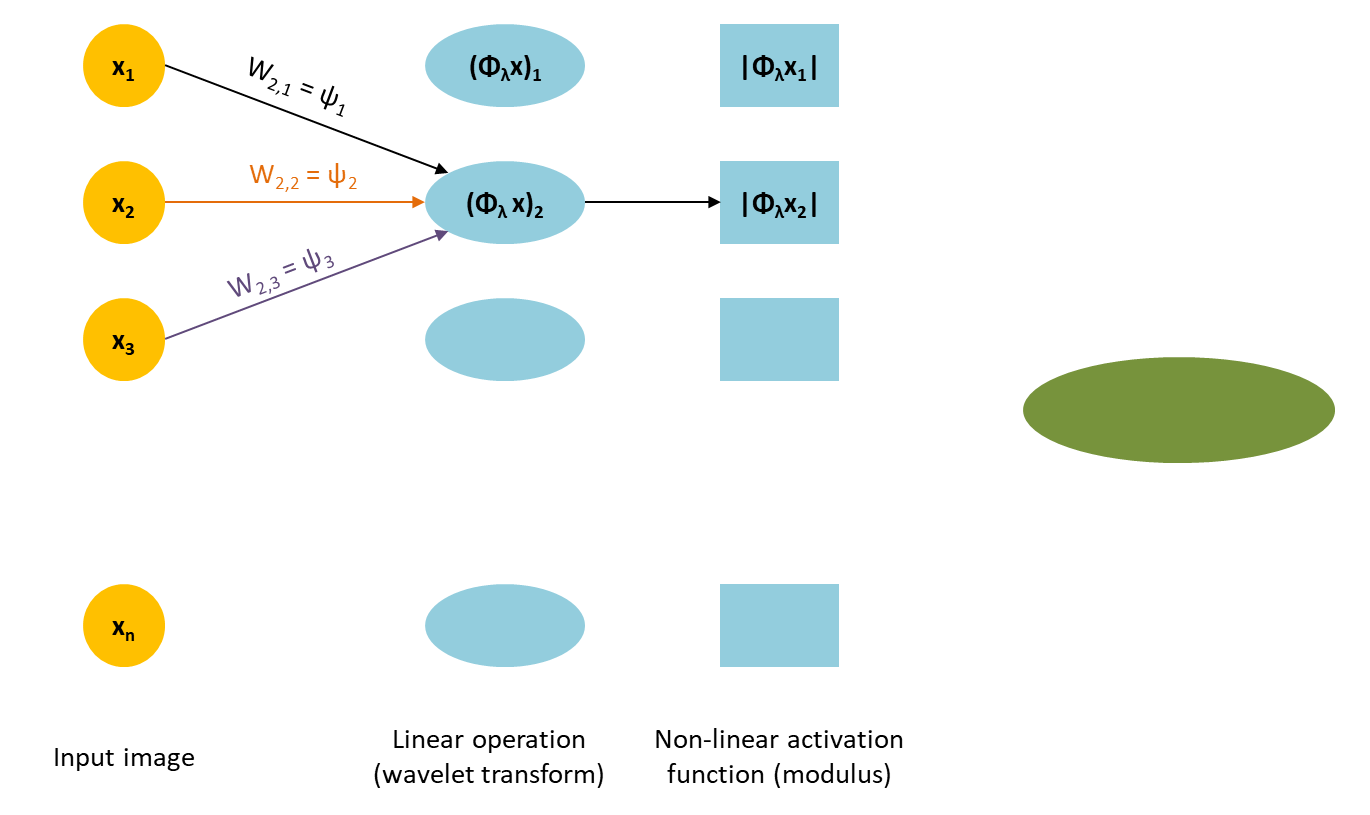
\includegraphics[width=\textwidth]{resources/convolution/CNN2.png}
    \end{figure}
    \end{frame}
    
    \begin{frame}{\subsecname}
    \framesubtitle{First convolution}
    \begin{figure}
        \centering
        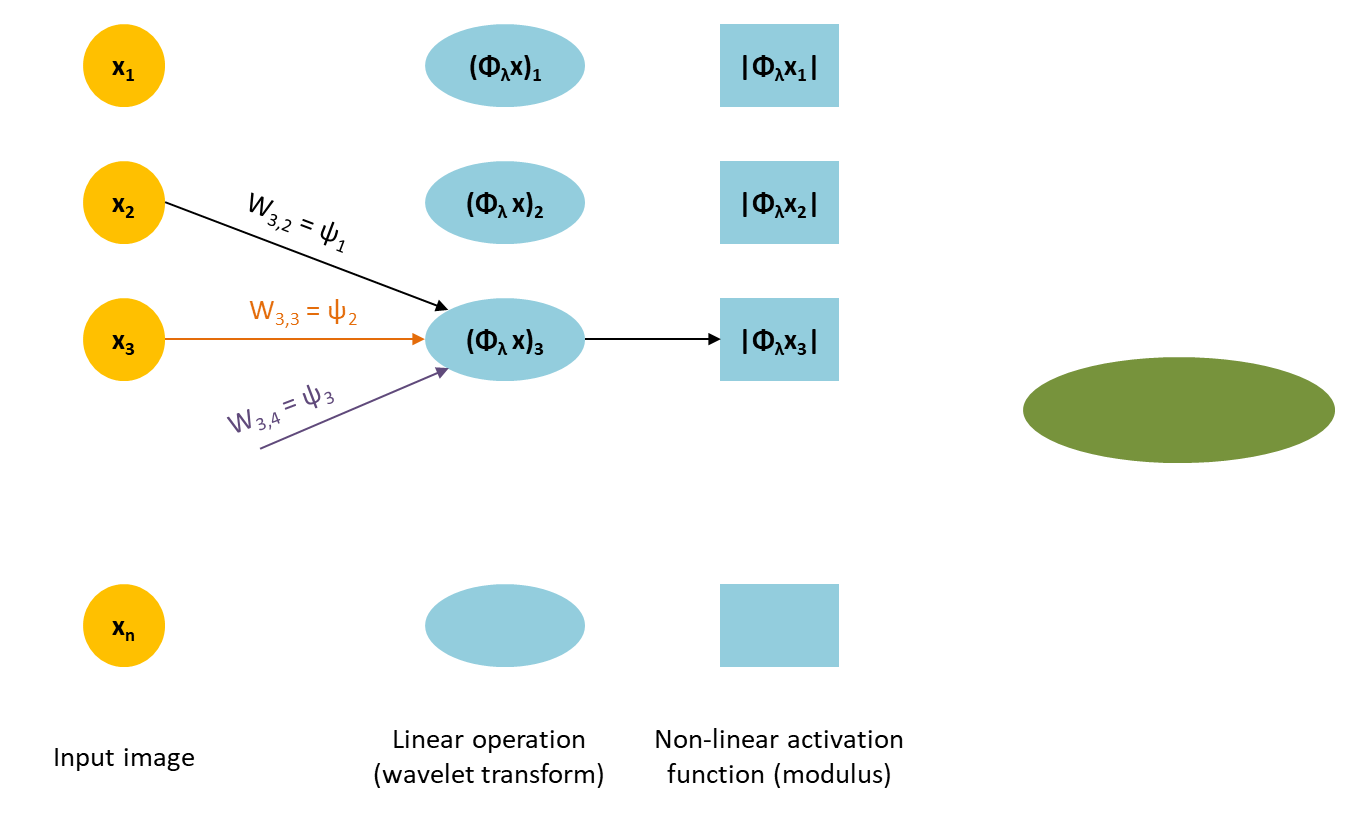
\includegraphics[width=\textwidth]{resources/convolution/CNN3.png}
    \end{figure}
    \end{frame}
    
    \begin{frame}{\subsecname}
    \framesubtitle{First convolution}
    \begin{figure}
        \centering
        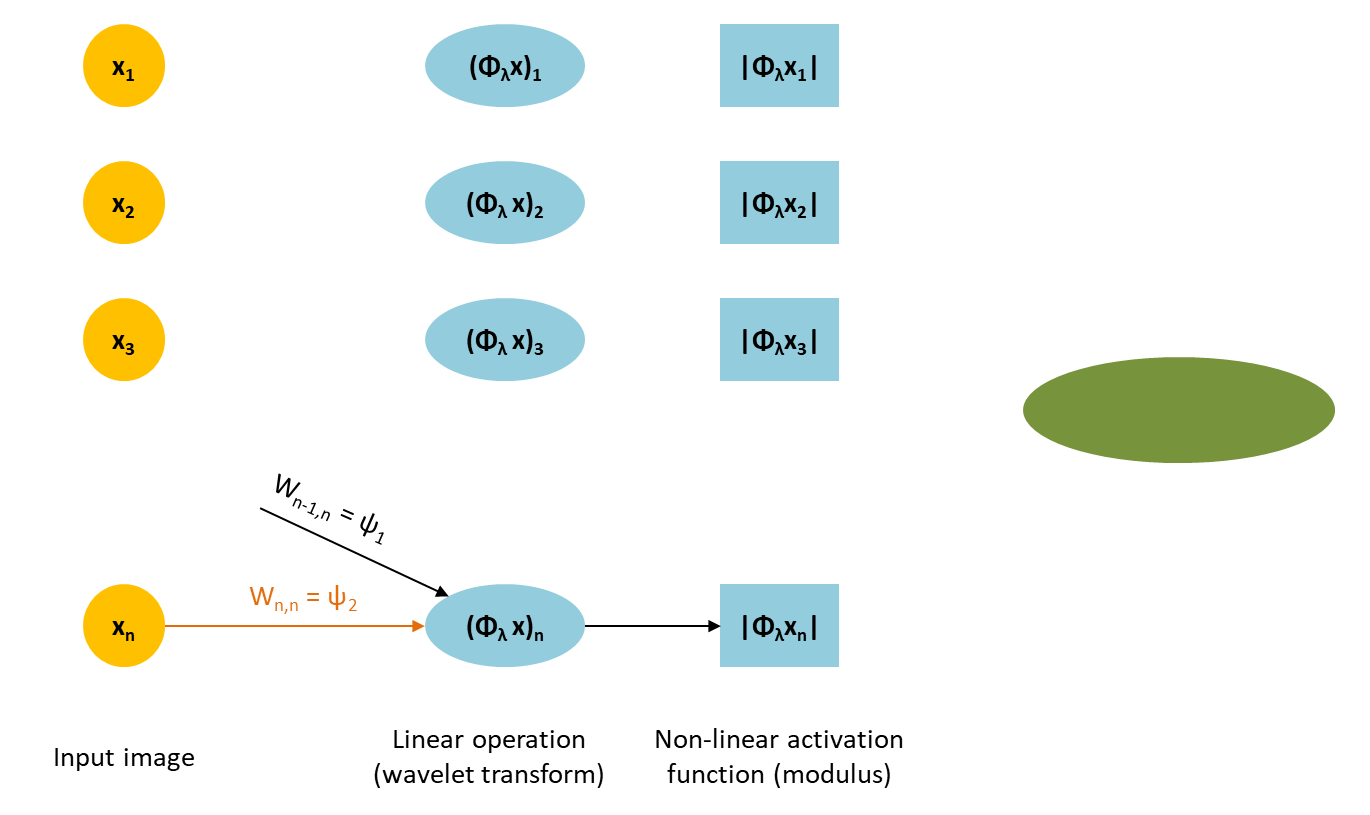
\includegraphics[width=\textwidth]{resources/convolution/CNN4.png}
    \end{figure}
    \end{frame}
    
    \begin{frame}{\subsecname}
    \framesubtitle{First convolution}
    \begin{figure}
        \centering
        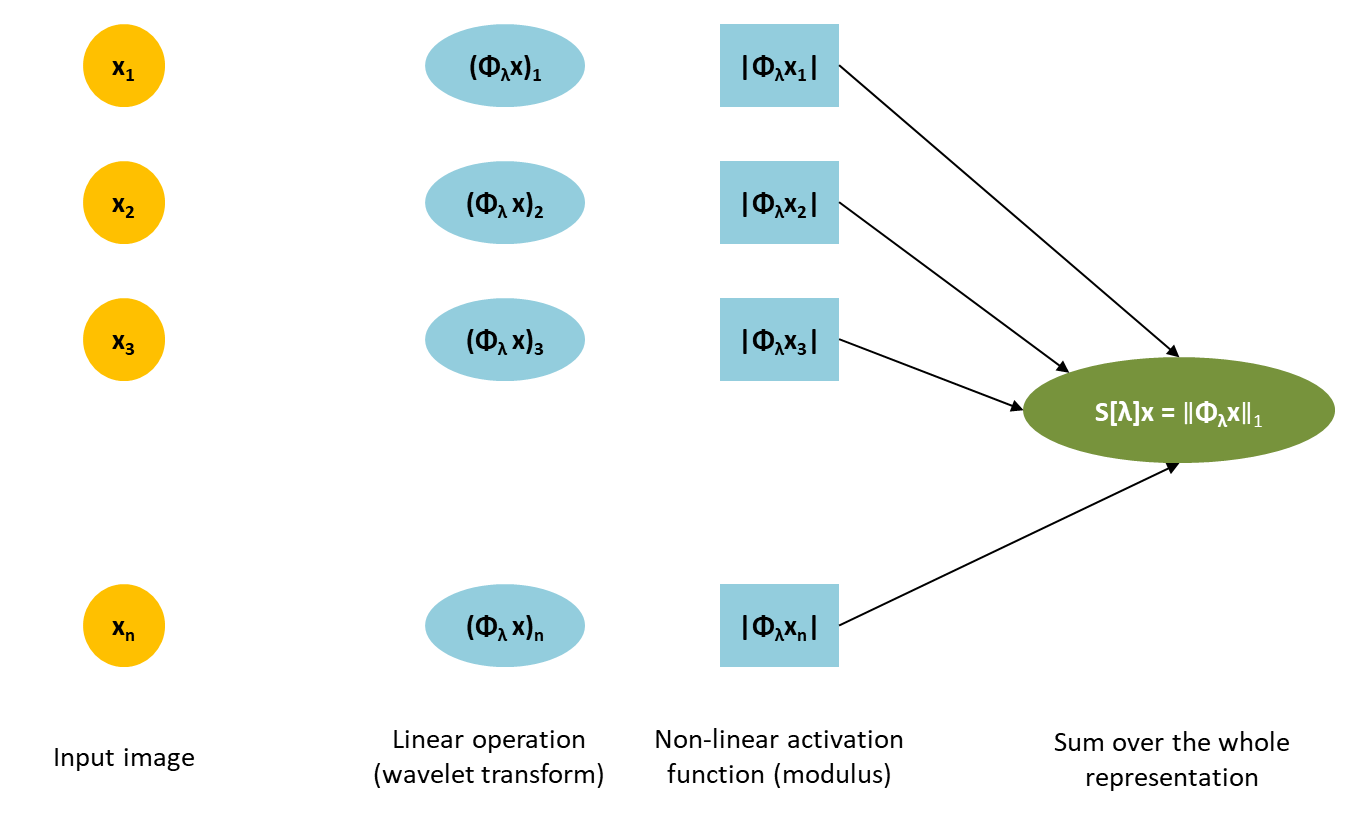
\includegraphics[width=\textwidth]{resources/convolution/CNN5.png}
    \end{figure}
    \end{frame}
    
    \begin{frame}{\subsecname}
    \framesubtitle{First convolution}
    \begin{figure}
        \centering
        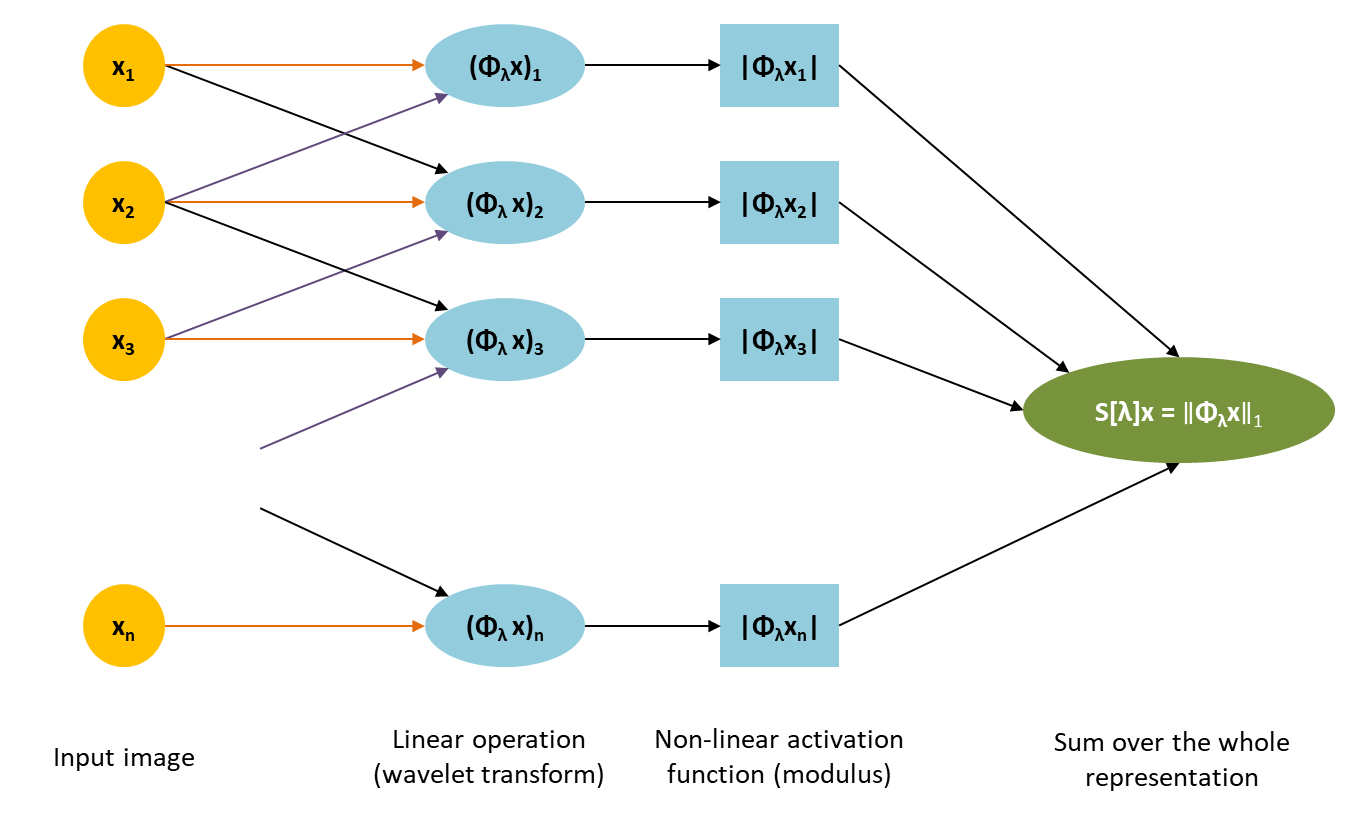
\includegraphics[width=\textwidth]{resources/convolution/CNN0.png}
    \end{figure}
    \end{frame}
    
    \subsection{Building a wavelet scattering network}
    
    \begin{frame}[label=build]{\subsecname}
    \begin{itemize}
        \item \col{Depth = 1:} we can compute as many invariants as parameters $\lambda = 2^{-j}r$, with $j \in \mathZ$ and $r$ being rotations of angles $2k\pi/K$, with $0 \leq k < K$:
    \end{itemize}
    $$x \longrightarrow \underbrace{|x \ast \psi_{\lambda_1}|}_{representation} \longrightarrow \underbrace{\|x \ast \psi_{\lambda_1}\|_1}_{invariant}$$
    \begin{itemize}
        \item \col{Depth > 1:} we can iterate the above procedure to build a deep convolutional neural network and compute powerful invariants:
    \end{itemize}
    \begin{equation}
    \begin{split}
        x \longrightarrow |x \ast \psi_{\lambda_1}|
            & \longrightarrow ||x \ast \psi_{\lambda_1}| \ast \psi_{\lambda_2}| \\
            & \longrightarrow ||||x \ast \psi_{\lambda_1}| \ast \psi_{\lambda_2}| \ast ...| \ast \psi_{\lambda_m}| \\
            & \longrightarrow \mbox{something comparable to } \|.\|_1
    \end{split}
    \end{equation}
    \end{frame}
    
    \begin{frame}[label=build]{\subsecname}
    \begin{itemize}
        \item For any depth $m$, we can define a \col{path:} $p = (\lambda_1, \lambda_2, ..., \lambda_m)$, along which iterative (non-linear) modulus wavelet transforms are computed:
    \end{itemize}
    \begin{equation}
    \begin{split}
        U[p]x
            & = ||||x \ast \psi_{\lambda_1}| \ast \psi_{\lambda_2}| \ast ...| \ast \psi_{\lambda_m}| \\
            & = U[\lambda_m] ... U[\lambda_2] U[\lambda_1] x
    \end{split}
    \end{equation}
    \begin{itemize}
        \item We compute a \col{wavelet scattering transform} along the path $p$, which can be compared to the $L1$-norm in the case of depth = 1:
    \end{itemize}
    $$\overline{S}x(p) = \mu_p^{-1} \int U[p]x(u) du$$
    with $\mu_p = \int U[p] \delta(u) du$ (normalization factor)
    \end{frame}
    
    \begin{frame}[label=build]{\subsecname}
    \begin{figure}
        \centering
        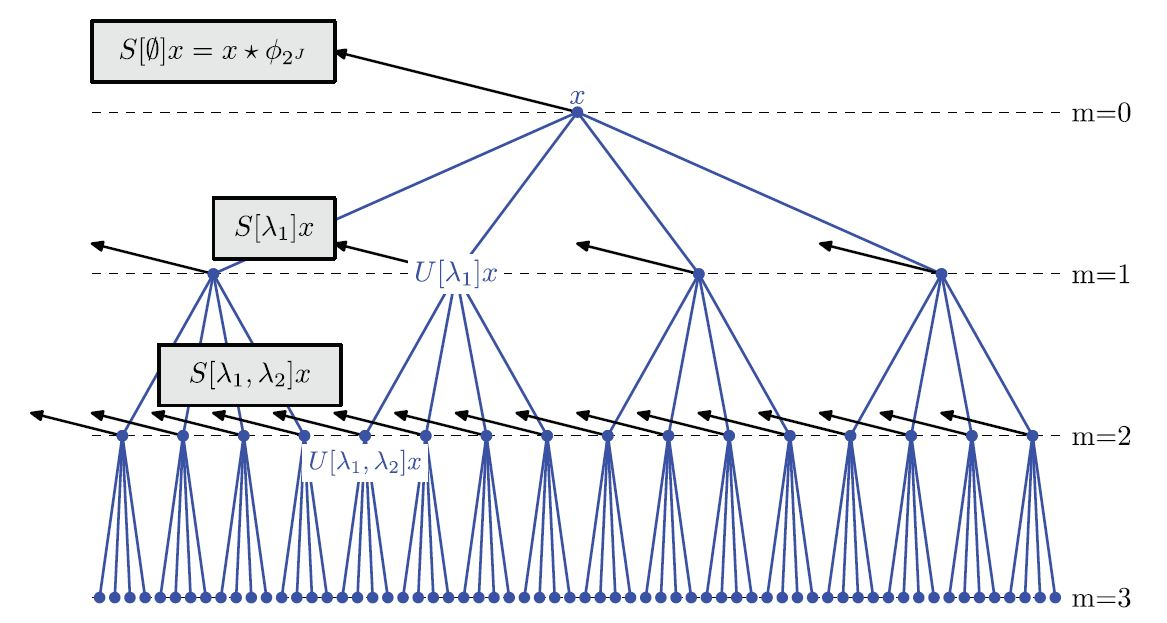
\includegraphics[width=\textwidth]{resources/convolution/Scattering_net.JPG}
        \caption{Representation of a wavelet scattering network with a depth equal to $m=3$. In this example, $1+4+16+64=85$ invariants are computed.\\Source: S. Mallat}
    \end{figure}
    \end{frame}
    
    \subsection{Scattering properties}
    
    \begin{frame}[label=scat_prop]{\subsecname}
    \end{frame}

  \end{darkframes}

\end{document}
